\chapter{O meu corpo}\label{ch:g1:my-body}

Fique na frente do espelho e acene: um corpo vivo inteiro acena de
volta. Ele vem crescendo desde antes de você nascer, dobra em alguns
lugares e em outros não, e é seu para a vida toda. Hora de olhar
para ele como olhamos para o gato e para a margarida --- parte por
parte.

\section{As partes do meu corpo}

\begin{definition}[Partes do corpo humano]\label{def:g1:my-body:parts}
O corpo humano tem três partes principais:
\begin{enumerate}
  \item a \emph{cabeça}\index{cabeça}, que carrega o rosto, os
        olhos, as orelhas, o nariz e a boca;
  \item o \emph{tronco}\index{tronco (corpo)}, o meio do corpo ---
        peito, barriga e costas;
  \item os \emph{membros}\index{membro}: dois \emph{braços}\index{braço}
        terminados em mãos, duas \emph{pernas}\index{perna}
        terminadas em pés.
\end{enumerate}
A cabeça fica sobre o \emph{pescoço}\index{pescoço}, que a liga ao
tronco.
\end{definition}

\begin{omfigure}
\begin{tikzpicture}
  \node[anchor=south west, inner sep=0] (img) at (0,0)
    {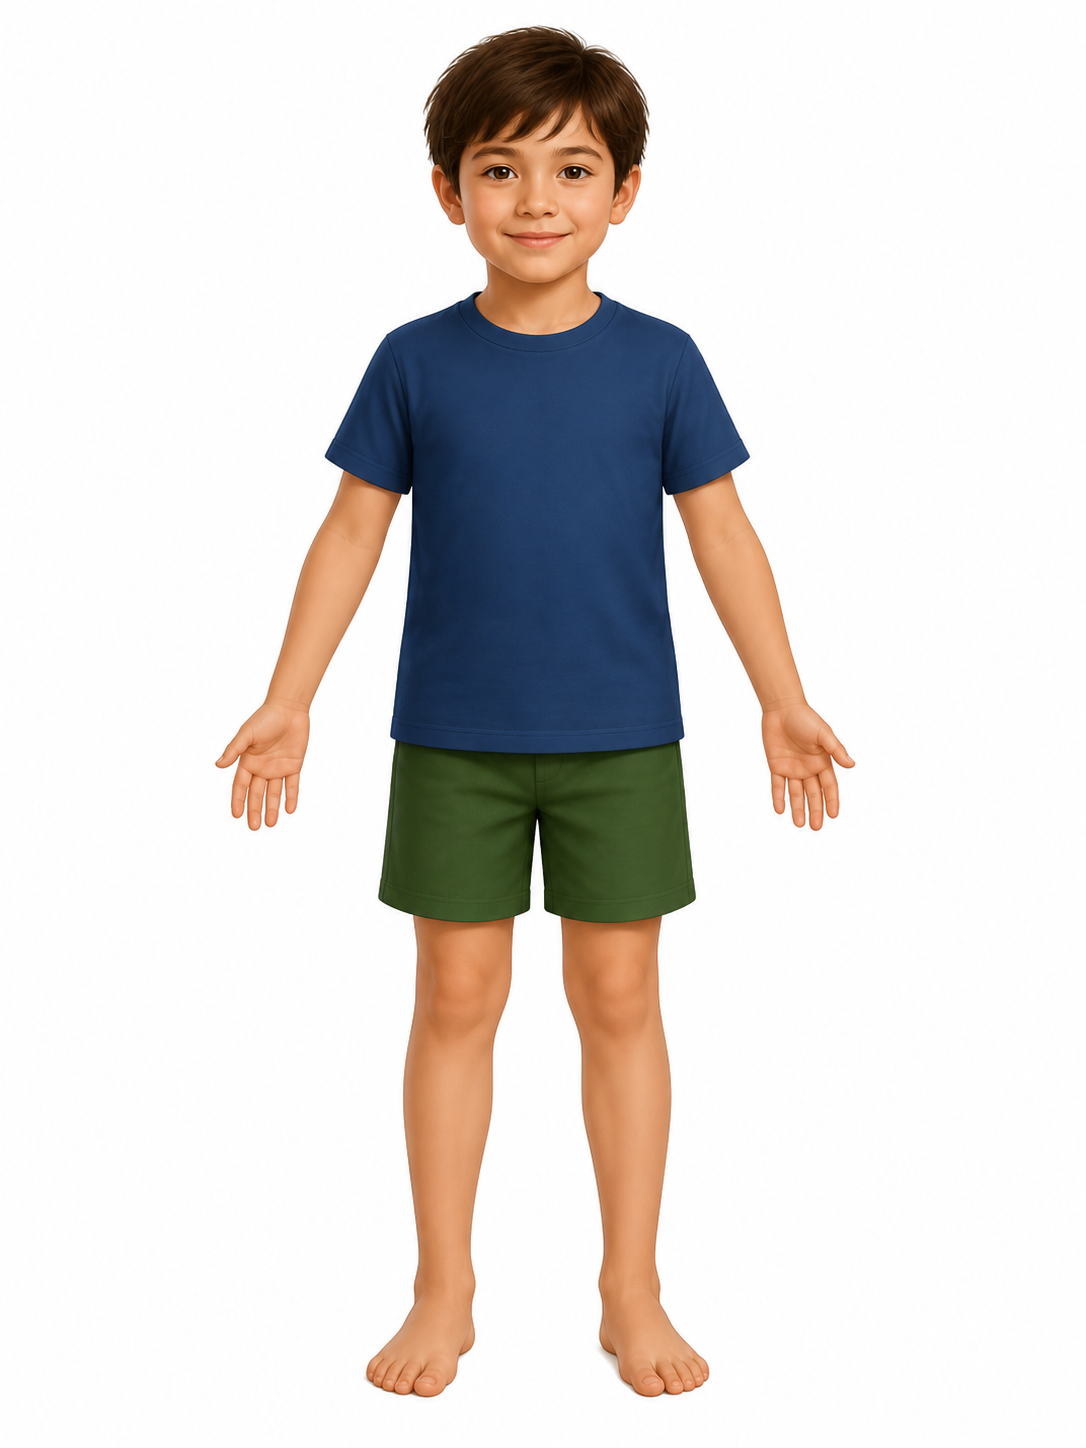
\includegraphics[width=0.42\linewidth]{images/book1/ai/fig-child-standing.png}};
  \begin{scope}[x={(img.south east)}, y={(img.north west)},
      every node/.style={font=\small}]
    \draw[omDef, thick] (0.57,0.90) -- (0.76,0.92) node[right] {cabeça};
    \draw[omDef, thick] (0.53,0.80) -- (0.76,0.83) node[right] {pescoço};
    \draw[omDef, thick] (0.58,0.62) -- (0.78,0.66) node[right] {tronco};
    \draw[omDef, thick] (0.74,0.46) -- (0.86,0.38)
      node[below, align=center] {braço e\\ mão};
    \draw[omDef, thick] (0.60,0.18) -- (0.78,0.14)
      node[right, align=left] {perna e\\ pé};
  \end{scope}
\end{tikzpicture}

{\small As três partes principais do corpo: cabeça, tronco e quatro
\omterm{def:g1:my-body:parts}{membros} --- com o pescoço ligando a cabeça ao tronco.}
\end{omfigure}

\begin{example}[O mesmo plano do gato?]\label{ex:g1:my-body:cat}
Compare-se com o gato: cabeça, corpo, quatro \omterm{def:g1:my-body:parts}{membros} --- o plano
parece igual. Mas o gato anda sobre as quatro patas; você fica em pé
sobre duas \omterm{def:g1:my-body:parts}{pernas} e mantém dois \omterm{def:g1:my-body:parts}{braços} livres para carregar,
desenhar e acenar. E, onde o gato tem cauda, você não tem nenhuma.
\end{example}

\section{Dobrar: as articulações}

\begin{definition}[Articulação]\label{def:g1:my-body:joint}
Uma \emph{articulação}\index{articulação} é um lugar onde o corpo
consegue dobrar ou girar. O \emph{cotovelo}\index{cotovelo} dobra o
\omterm{def:g1:my-body:parts}{braço}, o \emph{joelho}\index{joelho} dobra a \omterm{def:g1:my-body:parts}{perna}, o
\emph{ombro}\index{ombro} gira o \omterm{def:g1:my-body:parts}{braço} inteiro, o
\emph{punho}\index{punho} e o \emph{tornozelo}\index{tornozelo}
dobram a mão e o pé. Entre duas articulações, o corpo fica reto.
\end{definition}

\begin{omfigure}
\begin{tikzpicture}[scale=1.0]
  % straight arm
  \draw[very thick] (0,0) -- (2.0,0);
  \draw[very thick] (2.0,0) -- (3.8,0);
  \fill[omThm] (2.0,0) circle (0.1);
  \fill[omDef!60] (0,0) circle (0.1);
  \draw[thick, fill=omDef!8] (4.0,0) circle (0.18);
  \node[below, font=\small] at (1.9,-0.3) {braço esticado};
  % bent arm
  \begin{scope}[xshift=6.6cm]
    \draw[very thick] (0,0) -- (2.0,0);
    \draw[very thick] (2.0,0) -- (3.1,1.45);
    \fill[omThm] (2.0,0) circle (0.1);
    \fill[omDef!60] (0,0) circle (0.1);
    \draw[thick, fill=omDef!8] (3.22,1.6) circle (0.18);
    \node[below, font=\small] at (1.9,-0.3) {braço dobrado no cotovelo};
    \draw[omThm] (2.05,0.12) -- (1.55,0.8)
      node[above left, font=\small, omThm] {a articulação dobra};
  \end{scope}
  \node[font=\small] at (1.0,1.4) {ombro};
  \draw[omDef!60] (0.05,0.12) -- (0.55,1.15);
\end{tikzpicture}

{\small O \omterm{def:g1:my-body:parts}{braço} só dobra nas articulações: \omterm{def:g1:my-body:joint}{ombro} (azul) e \omterm{def:g1:my-body:joint}{cotovelo}
(vermelho). Entre eles, ele fica reto.}
\end{omfigure}

\begin{example}[Experimente: andar de joelho duro]\label{ex:g1:my-body:stiff}
Tente andar sem dobrar os \omterm{def:g1:my-body:joint}{joelhos}. Dá --- por pouco --- com passinhos
duros de pato. Agora tente pegar um lápis do chão sem dobrar \omterm{def:g1:my-body:joint}{joelhos},
quadris nem costas. São as articulações que deixam os movimentos do
corpo macios, rápidos e fáceis.
\end{example}

\begin{remark}[Direita e esquerda]\label{rem:g1:my-body:sides}
O corpo tem dois lados, direito e esquerdo, quase como um espelho:
um \omterm{def:g1:my-body:parts}{braço} e uma \omterm{def:g1:my-body:parts}{perna} de cada lado, um olho e uma orelha de cada lado
da cabeça. Saber diferenciar a mão direita da esquerda também é
conhecer o corpo --- é o que diz às pessoas para que lado você quer
apontar.
\end{remark}

\section{O meu corpo cresce}

\begin{proposition}[Crescer]\label{prop:g1:my-body:growth}
O corpo de uma criança \emph{cresce}\index{crescimento}: ele fica
mais alto e mais pesado, ano após ano, até o tamanho de adulto.
Crescer é lento e constante --- lento demais para sentir, fácil de
medir.
\end{proposition}
\admitted

\begin{example}[Marcas no batente da porta]\label{ex:g1:my-body:doorframe}
Encoste no batente da porta; um adulto marca a sua altura com um
lápis. Faça de novo alguns meses depois: a marca nova está mais
alta! Você nunca sentiu que estava crescendo, mas as duas marcas,
uma acima da outra, mostram isso com toda a clareza.
\end{example}

\begin{omfigure}
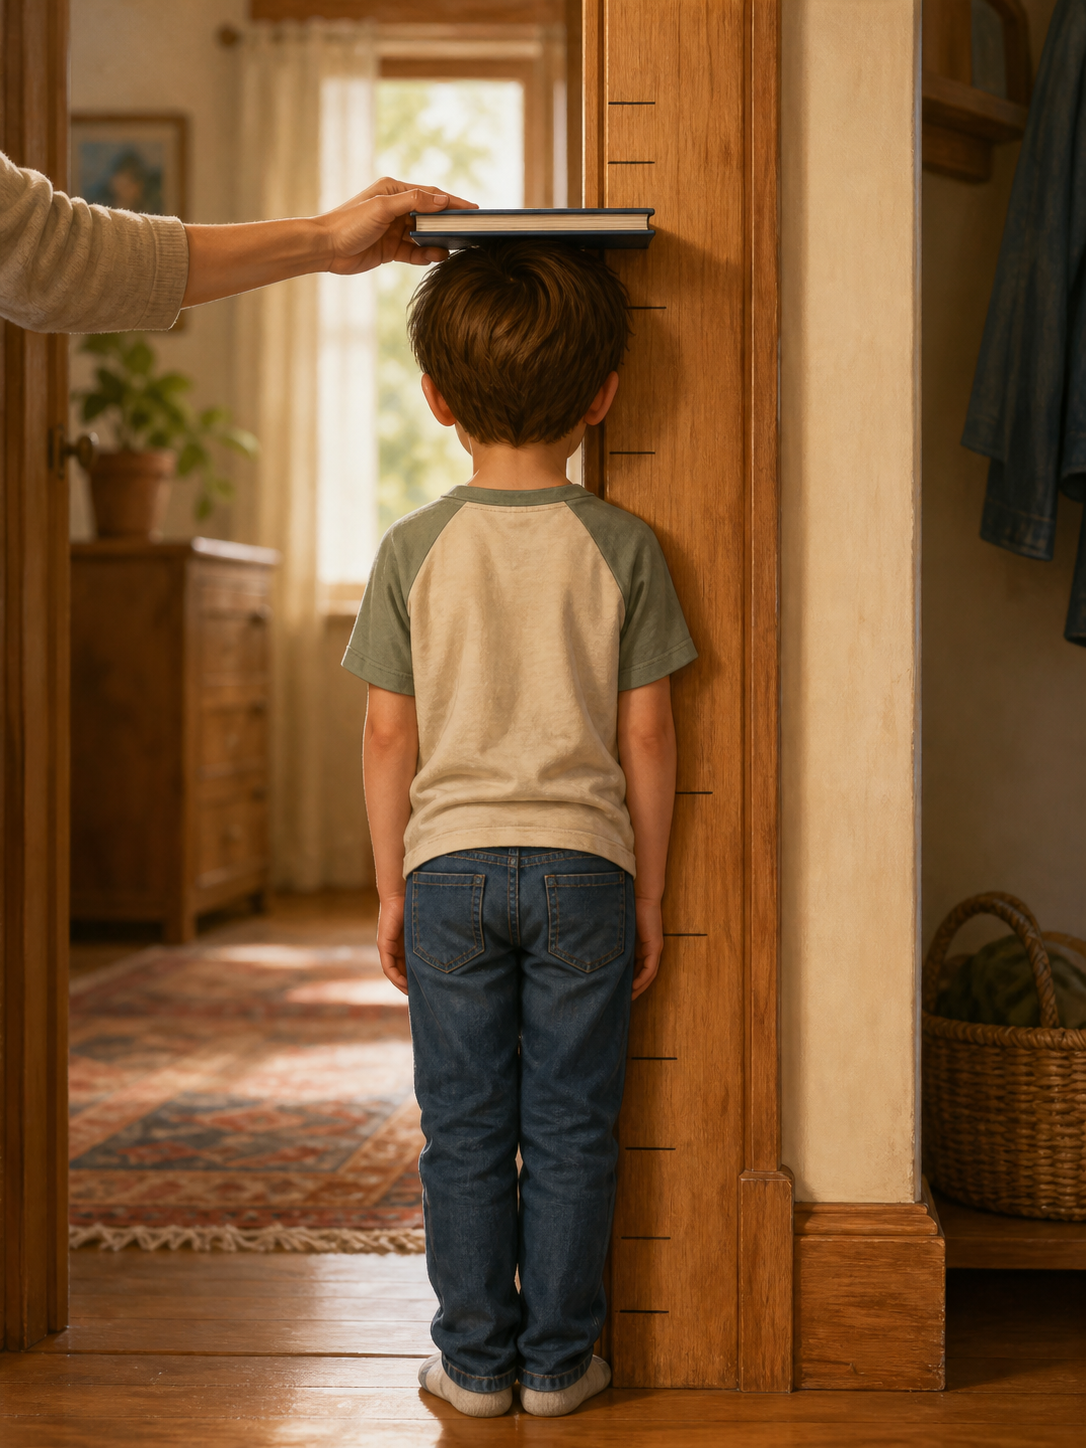
\includegraphics[width=0.46\linewidth]{images/book1/ai/g1-body-doorframe.png}

{\small Dia de medição no batente da porta: o livro deitado leva o
alto da cabeça direitinho até a madeira.}
\end{omfigure}

\begin{method}[Medir a minha altura]\label{met:g1:my-body:measure}
\begin{enumerate}
  \item Tire os sapatos;
  \item fique reto, com as costas e os calcanhares na parede,
        olhando para a frente;
  \item alguém apoia um livro deitado na sua cabeça, bem nivelado,
        encostando na parede;
  \item marque o ponto embaixo do livro e escreva a data ao lado.
\end{enumerate}
Medidas sempre do mesmo jeito, as marcas são confiáveis --- e dá
para compará-las.
\end{method}

\begin{remark}[Cada corpo é diferente]\label{rem:g1:my-body:different}
Numa mesma turma, algumas crianças são mais altas, outras mais
baixas; umas crescem mais cedo, outras mais tarde. Tudo isso é
normal. Os corpos são como os rostos: feitos no mesmo plano, e cada
um diferente. As marcas do seu batente são suas --- elas não servem
para competir com o vizinho.
\end{remark}

\section{Exercícios}

\begin{exercise}[$\star$]\label{exo:g1:my-body:1}
Diga as três partes principais do corpo humano. O que liga a cabeça
ao tronco?
\end{exercise}

\begin{exercise}[$\star$]\label{exo:g1:my-body:2}
Onde termina cada \omterm{def:g1:my-body:parts}{membro} --- o que fica na ponta de um \omterm{def:g1:my-body:parts}{braço}, e na
ponta de uma \omterm{def:g1:my-body:parts}{perna}?
\end{exercise}

\begin{exercise}[$\star$]\label{exo:g1:my-body:3}
Qual \omterm{def:g1:my-body:joint}{articulação} dobra: (a) o \omterm{def:g1:my-body:parts}{braço} no meio? (b) a \omterm{def:g1:my-body:parts}{perna} no meio?
(c) a mão na ponta do \omterm{def:g1:my-body:parts}{braço}?
\end{exercise}

\begin{exercise}[$\star$]\label{exo:g1:my-body:4}
Encoste a mão esquerda na sua orelha direita. Quais articulações o
seu \omterm{def:g1:my-body:parts}{braço} acabou de usar? Diga pelo menos duas.
\end{exercise}

\begin{exercise}[$\star$]\label{exo:g1:my-body:5}
No \cref{ex:g1:my-body:cat}, encontre um jeito em que o seu corpo é
parecido com o do gato e dois em que ele é diferente.
\end{exercise}

\begin{exercise}[$\star$]\label{exo:g1:my-body:6}
Por que a pessoa que ajuda no \cref{met:g1:my-body:measure} apoia um
livro deitado na sua cabeça em vez de só olhar?
\end{exercise}

\begin{exercise}[$\star$]\label{exo:g1:my-body:7}
Duas marcas no batente da porta: a do ano passado e a de hoje, um
pouquinho mais alta. O que as marcas mostram? Você sentiu isso
acontecendo?
\end{exercise}

\begin{exercise}[$\star$]\label{exo:g1:my-body:8}
Faça a experiência: ande de \omterm{def:g1:my-body:joint}{joelho} duro como no
\cref{ex:g1:my-body:stiff} e depois tente bater palmas sem dobrar os
\omterm{def:g1:my-body:joint}{cotovelos}. Que movimentos do dia a dia acabam precisando de
articulações?
\end{exercise}

\begin{exercise}[$\star\star$]\label{exo:g1:my-body:9}
A Mia é a menor da turma e fica preocupada com isso. O que a
\cref{rem:g1:my-body:different} responde para ela?
\end{exercise}

\begin{exercise}[$\star\star$]\label{exo:g1:my-body:10}
Um boneco feito de um único pauzinho de madeira não consegue sentar
numa cadeira. Onde você cortaria o pauzinho e poria pontos de girar
para ele conseguir sentar? Diga quais articulações do corpo os seus
cortes copiam.
\end{exercise}
